\cotefile{69}
\scanpage{68}
\diagram{\(\begin{array}{@{}r@{\ }l@{\quad}l}
 &\mathrm{Pl}(\unsure{L|D}_1,C)=C&27=3^3\\
 \uparrow&\mathrm{Pl}(L_2,C)&27.16=2^4 3^3=432\\
 \uparrow&\mathrm{Pl}(L_3,C)&27.16.10=2^5.3^3.5=4320\\
 \uparrow&\mathrm{Pl}(L_4,C)\xleftarrow{\sim}\mathrm{Pl}''(L_5,C)&27.16.10.6=2^6.3^4.5=25.920\\
 \unsure{\uparrow|\vert}&\mathrm{Pl}'(L_5,C)\unsure{:=|:}&27.16.10.6.2=2^7.3^4.5=51840\\
 2{\uparrow}&\mathrm{Pl}'(L_6,C&,5
\end{array}\)}

On trouve pour les configurations correspondantes

\diagram{\(\begin{array}{@{}l@{\quad}l@{\quad}l}
\deleted{\unsure{1|a}} B_1(C)&27:1=27=3^3&\mathrm{aut}\,L_1=e\\
B_2(C)&27.16:2!=27.8=2^3 3^3=216&\mathrm{aut}\,L_2\unsure{:|=}\unsure{\mathfrak S|\mathscr S}_2\\
B_3(C)&27.16.10:3!=2^{\deleted{\unsure{5|3}}4}.3^2.5=720=6!&\mathrm{aut}\,L_3=\mathfrak S_3\\
B_4(C)&27.16.10.6:4!=2^3.3^3.5=1080&\mathrm{aut}\,L_4=\mathfrak S_4\\
\quad\unsure{\simeq|\approx} B_4''(C)&&\\
B'_5(C)&27.16.10.6.2:5!=2^4.3^3=432&\mathrm{aut}\,L_5=\mathfrak S_5\\
B(C)=B_6(C)&27.16.10.6.2.1:6!=2^3 3^2=72&\mathrm{aut}\,L_5\simeq\mathfrak S_6\\
\mathrm{Bib}(C)&36&\mathrm{aut}(L'_5)\simeq\mathfrak S_2\times\mathfrak S_6
\end{array}\)}

\begin{center}\rule{1.5cm}{.5pt}\\[-.8ex]\rule{1.1cm}{.4pt}\end{center}

\uline{Étude cas par cas}

1) $\mathrm{Pl}(L_1,C)=C$ \inserted{de cardinal $27$}. Si $x\in C$, $\mathrm{Aut}(C;x)$ est transitif sur l'ens \deleted{\unsure{des|de}} $C-\Xi(x)$ \inserted{de cardinal $16$} \deleted{[\unsure{des pts} $z\ne x$ \unsure{liés|à $x$}]}.

2) $\mathrm{Pl}(L_2,C)$

\uline{Prop.} Pour \unsure{deux|des|tout} couples $(x,y)$ de sommets dist. non liés, $\exists!$ base $b$ telle que $x\in b$, $y\in b'$ \inserted{base opposée} (et $x,y$ \deleted{liés} correspondent $y=\sigma_b\unsure{x=\sigma_{b'}x|x\Rightarrow\sigma_{b'}x}$, $x=\sigma_b y=\sigma_{b'}y$)

Ainsi l'ens des \deleted{couples} \inserted{parties gauches 2-libres} $(x,y)$ \deleted{de sommets} est en corr. $1$--$1$ avec l'ens des couples d'une base $b$ et d'un $x\in b$. La cat. des $(C,(x,y))$ équivaut à celle des ens. de cardinal $5$ (\unsure{ou encore}, des ens de cardinal $6$ à pt marqué)

On peut écrire $(x,y)=(\unsure{\delta_6|\delta_\sigma|J_\sigma|\xi_6},\delta'_6)$. L'ens $C-\Xi(\delta_6)-\unsure{\Sigma|\Xi|E}(\delta'_6)$ \inserted{$-\{x\unsure{+|,}y\}$} des pts \inserted{$\ne x,y$} non liés, ni à $y$ est l'ens des $\delta_{ij}$ $(1\leq i<j\leq5)$, de cardinal $10$ \inserted{$=\binom{5}{2}$}, et $\mathrm{Aut}(C,(x,y))=\mathfrak S_5$ y opère transitivement.
% archive sheet number: 67
\scanpage{69}
Cas des paires $\{x,y\}$ de pts dist. non liés. La donnée équivaut à une \uline{bibase} $B=\{b,b'\}$ avec un elt $z$ de $B/\sigma_B=I$. La catégorie des $(C,\{x,y\})$ équivaut à celle des couples $(\tau,J)$ de deux ens avec $\tau$ de cardinal $2$, \inserted{$(\tau=\{b,b'\})$} $J$ de cardinal $5$ ($J=B/\sigma_B-\{z\}$).
\margin{$\unsure{\widehat{\mathrm{Ens}}_2|\mathrm{Ens}_2}\times\widehat{\mathrm{Ens}}_5$}
% slanted
\noindent\rule{2.3cm}{.4pt}

$\uline{\mathrm{Pl}}(L_3,C)$. Le type d'une partie \inserted{épinglée} trois-libre \inserted{$(x,y,z)$} de $C$ est $(\unsure{\delta_{12}|J_{12}|\xi_{12}},\delta_{23},\delta_{31})$. L'ens des pts de $C-\{\{\delta_{12},\delta_{23},\delta_{31}\}$ qui ne sont \deleted{pas} liés \deleted{aux} \inserted{d'aucun} des $x,y,z$ est $\{\underbrace{\delta_4,\delta_5,\delta_6},\underbrace{\delta'_{\unsure{45|4}},\delta'_{\unsure{56|5}},\delta'_{\unsure{65|6}}}\}$ qui est de

cardinal $6$; le groupe des autom. de $(C;\delta_{12},\delta_{23},\delta_{31})$ (contenant le groupe des autom de $(C,\{\{\delta_i\}\},\{\delta'_i\})$ qui respecte la partition \inserted{de $b\unsure{=|\simeq}$} $[1,6]$ en $[1,3]$ et $[4,6]$) est transitif sur l'ens précédent.

\uline{Prop} Pour tt couple \inserted{$(B,K)$} formé d'une bibase $B=\{b,b'\}$ \inserted{de $C$} et d'une partie $K$ de $B/\sigma_B$ telles que $\mathrm{Card}\,K=3$, soit $J(B,K)$ l'ens partie de $C$ formée les $\delta^B_{ij}$ $(i,j\in K)$. On trouve ainsi une bijection de l'ens \deleted{\unsure{d|l|$\mathcal B$}} de cardinal $72.\underbrace{\binom{6}{3}}_{20}\frac{1}{2}=720)$ des couples $(B,K)$ avec l'ens des parties $3$-libres de $C$.

La cat. des couples $(C,J)$ d'un graphe cubique et d'une partie $3$-libre de $C$, équivaut donc à celle des triplets $(\tau,K,K')$ d'ens \margin{$\widehat{\mathrm{Ens}}_2\times\widehat{\mathrm{Ens}}_3\unsure{\times|-}\widehat{\mathrm{Ens}}_3$} de cardinal $2,3,3$ -- en associant à un triple le complexe $C=\unsure{\mathbb E|\mathscr E|C}(\tau,K\amalg K')=(\tau\times(K\amalg K'))\amalg\unsure{\mathfrak P_2|\mathscr P_2}(K\amalg K')$, et l'ens $J$ des $\delta^B_{ij}$ $(i,j\in K)$, où $B$ est la bibase can. de $C$. Le groupe
% slanted
% archive sheet number: 68
\scanpage{70}
des autom des $(C,J)$ est donc \unsure{can$^{\mathrm{t}}$.|can$^{\mathrm{t}}$,}
\[
:\quad \unsure{\mathfrak S|\mathscr S}_\tau\times\mathfrak S_K\times\mathfrak S_{K'}\quad(\simeq\mathfrak S_2\times\mathfrak S_3\times\mathfrak S_3]
\]
d'ordre $72$.

\uline{NB} Il y a une involution naturelle dans cette catégorie des $(\tau,K,K')$, savoir
\[
(\tau,K,K')\longmapsto(\tau,K',K)
\]
Elle se traduit en associant à $(C,J)$ le $(C,J')$, où $J'$ est l'ens de cardinal $3$ des éléments de $C$ liés à tous les él. de $J$. Dans le cas où
\[
J=\{\unsure{\delta_{12}|J_{12}|\xi_{12}},\delta_{23},\delta_{31}\},\quad\text{on a}\quad J'=\{\delta_{45},\delta_{56},\delta_{\unsure{61|64}}\}.
\]

\uline{Corollaire.} $J$ appartient à \unsure{exactmt|exactement} $2$ bases, \deleted{(dans le cas envisagé, $\{\delta_{12},\delta_{23},\delta_{\unsure{34|31}}$ \unsure{prolongé|prolongés} soit} \inserted{savoir $J\cup(b\vert K')$ et $J\cup(b'\vert K')$} (dans \unsure{l'exp.|l'ex.} le \unsure{voisin|voisinage|réunion} de $J=\{\delta_{12},\delta_{23},\delta_{31}\}$ avec $\{\delta_4,\delta_5,\delta_6\}$ ou $\{\delta'_4,\delta'_5,\delta'_6\}$) dont l'intersection est réduite à $J$. \deleted{Ainsi}

Considérons alors l'application $\{\beta',\beta''\}\longrightarrow\beta'\cap\beta''$ de l'ens des couples de bases telles que $\mathrm{card}\,\beta'\cap\beta''=\underline{3}$, vers l'ens des parties $3$ libres de $C$, cette application est encore bijective. Cet ens s'identifie aussi à l'ens des paires $\{r,s\}$ de racines telles que $\widehat{r,s}=60^\circ$.
\margin{\unsure{expliciter|explicitez} position relative de $2$ racines}
% slanted
% archive sheet number: 69
\scanpage{71}
\uline{Corollaire} (cf plus bas) Pour tte partie $3$-libre $J$ de $C$, l'ens $\unsure{\mathscr L|L|\mathcal L}(J)$ des él. de $C-J$ non liés aux él. de $J$, est un \uline{hexagone}, et on trouve ainsi une corr. biun. entre $B_3(C)$ et l'ens $\mathrm{Hex}(C)$ des hexagones dans $C$; l'application inverse associe à un hexagone $H$ l'ens $\mathscr L(H)$ des els de $C-H$ non liés aux él. de $H$.
\diagram{\begin{tikzcd}[ampersand replacement=\&,row sep=1.1em,column sep=.75em]
\& |[label=above:{$\unsure{\delta'_6|J'_6|\xi'_6}$}]|\bullet \arrow[-]{r} \arrow[-]{dl} \arrow[-,dashed]{dd} \arrow[-,dashed]{drr}
\& |[label=above:{$\delta_4$}]|\bullet \arrow[-]{dr} \arrow[-,dashed]{dd} \arrow[-,dashed]{dll} \& \\
|[label=left:{$\delta_5$}]|\bullet \arrow[-]{dr} \arrow[-,dashed]{drr} \& \& \&
|[label=right:{$\delta'_5$}]|\bullet \arrow[-]{dl} \arrow[-,dashed]{dll}\\
\& |[label=below:{$\delta'_4$}]|\bullet \arrow[-]{r} \& |[label=below:{$\delta_6$}]|\bullet \&
\end{tikzcd}}

\uline{NB} La donnée d'un graphe hexagonal ($=$ hexagone combinatoire) équivaut à celle d'un couple \deleted{d'ens} $(\tau,K')$ d'un ens de card $2$ et d'un autre de cardinal $3$ (l'hexagone étant alors $\tau\times K'$, deux sommets étant liés ssi ils \deleted{ne sont pas} ont des \deleted{\unsure{projections|projecteurs}} \inserted{composantes} distinctes dans $\tau$ et dans $K'$, i.e. ssi \unsure{ils proviennent} d'un elt de $\tau\times K'$ qui ils \deleted{forment} est le graphe d'une \unsure{imm.|invers.} $\tau\hookrightarrow K'$). Ceci dit, si $(C,J)$ est défini par $(\tau,K,K')$, l'hexagone contenu dans dans $C$ est défini par $(\tau,K')$, ou mieux $\tau\times K'\subset B=\deleted{\unsure{\{b,b'|\{b\cup b'}}\tau\times(K\amalg K')$ \ldots.

\uline{Parties $4$ libres} Cas typique $J=\{\delta_1,\delta_2,\delta_3,\delta_4\}$; $\mathscr L(J)=\{\delta_5,\delta_6,\delta_{56}\}$. \margin{$\unsure{\widehat{\mathrm{Ens}}_2|\mathrm{Ens}_2}\times\widehat{\mathrm{Ens}}_4$} On sait par l'étude précédente que $J$ est contenu dans une base \uline{unique} $b$, et $b\cap \mathscr L(J)$ est év. de cardinal $2$ (c'est $\{\delta_5,\delta_6\}$, il reste un pt dans le \unsure{complém.|complém} ($\delta_{56}$). Donc $\mathrm{Aut}(C,J)$ (ou à fortiori $\mathrm{Aut}(C,\delta_1,--,\delta_4)$) n'opère pas transitivement sur $\mathscr L(J)$, mais \deleted{$\mathscr L(J)$} a deux orbites $b\cap \mathscr L(J)$ ($=\{\delta_5,\delta_6\}$) et le pt fixe $\{\delta_{56}\}$.
% slanted

Donc $\deleted{\unsure{B|\mathrm{Pl}}}\mathrm{Pl}'(L_5,C)\to\mathrm{Pl}(L_4,C)$ est de degré $2$, et $\mathrm{Pl}''(L_5,C)\to\mathrm{Pl}(L_4,C)$ de degré $1$. Notons que l'ens $E(J)$ des el de $C$ liés à \unsure{un|nul|tt} él. de $J$ est de cardinal $2$ (c'est $\{\delta'_5,\delta'_6\}=\unsure{b'-|\}b'|b'\cap}\sigma_b(J)$ \deleted{\unsure{$\mathscr L(J)\to$}}), et on a une bijection canonique (induite par $\sigma_b$)
\[
E(J)\simeq (b-\!J)=b\cap \mathscr L(J)\subset \mathscr L(J)
\]

\uline{Parties $5$ libres} $1^{\mathrm o})$ Celles qui sont contenues dans une base, sont contenues dans une base unique\inserted{-- ce sont les $\mathscr L(J)$ de cardinal $1$ ($=\{\delta_6\}$), et aussi $E(J)$ ($=\{\delta'_6\}$).}
\margin{$\widehat{\mathrm{Ens}}_5$\quad La cat. des $(C,J)$, $J$ une $5$-libre, équivaut \deleted{au \unsure{i}} à celle des \deleted{couples $(C,\unsure{J|j})$ d'une partie de card. $2$, et d'une autre} ens $J$ de card $5$.}
% slanted
$2^{\mathrm o})$ Pour les autres, on vérifie que ce sont des $\unsure{\frac12|4_2|2}$ étoiles.

\uline{Prop.} L'application qui, à tte paire $\{x,y\}$ de pts non liés de $C$, associe $E(x)\cap E(y)$, est une bijection de l'ens de ces paires avec l'ens des $\frac12$ étoiles (parties $5$-libres ne s'immergeant pas dans une base). \inserted{La bijection inverse est $J\longmapsto E(J)$} Si on tient compte de $\{x,y\}\longleftrightarrow(\text{bibase }B=\{b,b'\},\text{ avec }z\in B/\sigma_B)$,
% archive sheet number: 70
\scanpage{72}
On trouve que $J=\{\unsure{\delta^B_{z,i}|J^B_{z,i}|\xi^B_{z,i}}\}_{i\in I-\{z\}}$ -- en \unsure{termes|types} de base $(\delta_i)_{1\leq i\unsure{<|\leq}6}$, $\unsure{\dot z|z}=(\delta_6,\delta'_6)$, $J=\{\delta_{i6}\}_{1\leq i\leq5}$. La cat. des \deleted{$\frac12$ étoiles} couples $(C,J)$, $J$ une $\frac12$ étoile, est donc équivalente à celle des couples $(\tau,J)$, $\tau$ ens de card $2$, $J$ ens de card. $5$.
\margin{$\unsure{\widehat{\mathrm{Ens}}_2|\mathrm{Ens}_2}\times\widehat{\mathrm{Ens}}_5$}

\uline{Bases et bibases} (Il fallait commencer par \unsure{ça|là}!)
\margin{$\widehat{\mathrm{Ens}}_6$}
\margin{$\widehat{\mathrm{Ens}}_2\times\widehat{\mathrm{Ens}}_6$}
% slanted
$W=\mathrm{Aut}(C)$ est simplement transitif sur l'ens des bases épinglées ($=$ ordonnées). Il y a $72$ bases, le groupe de stabilité d'une base est $\simeq\unsure{\mathfrak S|\mathscr S}_6$. Il y a $36$ bibases, groupe de stabilité $\mathfrak S_2\times\mathfrak S_2$.
La cat. des $(C,b)$ est $\simeq$ celle des ens. de card $6$, celle des $(C,B=\{b,b'\})$ à celle \unsure{des|ses} couples $(\tau,I)$, $\tau$ ens de cardinal $2$, $I$ ens de cardinal $6$.
% archive sheet number: 71
\scanpage{74}
1) \uline{Bitriangle} $\Delta$ : \inserted{graphe} isomorphe au \inserted{graphe} produit de deux triangles : $\Delta\simeq s\times t$, \inserted{($\mathrm{Card}\,s=\mathrm{card}\,t=3$)} \inserted{$x=(\alpha,\beta)$ et $x'=(\alpha',\beta')$, \inserted{$x\ne\unsure{y|x'}$} liés ssi $\alpha=\alpha'$ ou $\beta=\beta'$ \deleted{($x\ne x'$)}} \deleted{\unsure{2)}} donc $9$ sommets et $4.9:2=18$ arêtes.
Les triangles $\subset\Delta$ sont les $6$ fibres des deux projections $s\times t\ \substack{\longrightarrow s\\\longrightarrow t}$, \inserted{soit $T$ leur ens,} ils se groupent en deux familles par la relation \textquotedblleft$p\simeq q$'' ssi $p=q$ ou $p\cap q=\varnothing$ ($\Longleftrightarrow\mathrm{card}\,p\cap q\ne1$) L'ens des classes, $\tau$, donne lieu à un rev. d'ordre $3$ $T\longrightarrow\tau$ ($\mathrm{card}\,\tau=2$).
La cat. des $\Delta$ équivaut à celle des ens $T$ de cardinal $\unsure{5|6}$ munis d'une partition de type $(3,3)$, ou encore, des flèches de degré $3$ $T\longrightarrow\tau$ de $\mathrm{Ens}$, avec $\mathrm{card}\,\tau=2$. On associe à $T\longrightarrow\tau$ le graphe $\Delta=\prod_{i\in\tau}T_i$, avec \deleted{les arêtes} $x,y$ \inserted{$\in\Delta$} liés ssi $x\ne y$ et \deleted{\unsure{$x_i$|$y$}} $\exists\,i\in\tau$ tel que $x_i=y_i$ (ou encore, ssi $\exists!\,i\in\tau\quad x_i=y_i$).

2) \uline{Le bloc de triades} C'est un graphe \deleted{\unsure{$\Delta$|$D$}} $D$ tel que le graphe opposé $\overline D$ ($(x,y)$ liés \inserted{dans $\overline D$} ssi $x\ne y$ et $x,y$ \uline{non liés} dans $D$) soit un bitriangle. Ainsi $D=c\times d$, $\mathrm{card}\,c=\mathrm{card}\,\unsure{t|d|T}=\unsure{d|3}$, avec $x=(\lambda,\mu)$ et $\unsure{y'|x'}=(\lambda',\mu')$ liés sss : $\lambda\ne\lambda'$, $\mu\ne\mu'$. Il y a donc.
$\deleted{\frac{\mathrm{card}(D\times D-D)}{2}}\inserted{\binom{\mathrm{card}\,D}{2}}-18=\deleted{\text{arêtes}}18$ arêtes, \unsure{ô|,} tiens tiens, le \unsure{même nb|m. nb} que pour le bitriangle $\overline D$. Il y a $6$ triades i.e. \deleted{\unsure{triplets de}} \inserted{parties} de cardinal $3$ formées de pts mutuellmt non liés, soit $S$ leur ens, se groupant en $2$ familles de $3$, d'où rev. de degré $3$ $S\to\sigma$ ($\mathrm{card}\,\sigma=2$).

\uline{Proposition} Le bloc de triades est isom. à un bitriangle -- i.e. si $\Delta$ \inserted{$=s\times t$} est un bitriangle, $\Delta\simeq\overline\Delta$.

\uline{Dém} On va définir dans $\Delta$ une autre famille $S$ de $6$ parties à trois éléments -- savoir l'ens \inserted{$S$} des triades $\subset\Delta$. Ce sont aussi les parties \inserted{$u$} de $\Delta=s\times t$ \inserted{de cardinal $3$} telles que les deux projections $u\to s$ et $u\to t$ soient injectives (donc bijectives) donc ce sont les graphes des bijections $s\xrightarrow{\sim}t$ -- il y en a en $6$.
Elles se groupent en $2$ familles de trois éléments, en prenant \deleted{les} la relation $\varphi\sim\psi$ ssi $\varphi^{-1}\psi\deleted{^{\unsure{+|\ast}}}$ est une permutation paire de $s$ \deleted{condition} [$S$ \inserted{$=\mathrm{Isom}(s,t)$} est un torseur sous \deleted{$\mathrm{Isom}$ Aut} $\mathrm{Aut}\,s=\unsure{\mathfrak S|\mathscr S}_s$, et on prend les \inserted{$2$} classes sous le sous-groupe d'indice $2$ $\mathfrak S_s^{\unsure{+|\ast}}$; on voit que ce partage ne dépend pas de l'ordre dans lequel on prend $s,t$ \unsure{\ldots|ou}
% archive sheet number: 73
\scanpage{75}
Si $\varphi,\psi$ \inserted{$\in S_i$ ($i\in\sigma$)} sont dans une $=$ classe \inserted{$i\in\sigma$} et $\varphi\ne\psi$, on a $\varphi\cap\psi=\varnothing$ i.e. $\varphi^{-1}\psi$ sans pt fixe (en effet, c'est une des deux perm. circ. de $s$) donc les \inserted{trois} $\varphi\in S_i$ forment une \uline{partition} de l'ens $\Delta$ de cardinal $9$. De $\overline{\unsure{m|=}}$ pour l'ens $S_j$ ($j\in\sigma$, $j\ne i$). On trouve ainsi une application
\[
\Delta\xrightarrow{\sim}\prod_{i\in\sigma}S_i
\]
je dis qu'elle est bijective. \deleted{\unsure{Il|Le}}\unsure{Cela|Il} revient au $=$ de dire qu'elle est injective, ou encore de dire qu'un él. $(\alpha,\beta)$ de $\Delta=s\times t$ est connu quand on connaît ses deux composantes dans $S_i\times S_j$ ($\sigma=\{i,j\}$). Choisissons un isom $s\simeq t$, d'où un isom $\sigma\simeq\{1,2\}$, \deleted{\unsure{$\Delta$|et}} \inserted{$\Delta\to\underset{\text{''}S_1}{c}\times\underset{\text{''}S_2}{d}$,} il revient au $=$ de dire qu'un couple $(\alpha,\beta)$ d'él. de $s$ est connu quand on connaît l'unique permutation circulaire $\rho_1$ telle que $\beta=\rho_1\alpha$ (ceci détermine $\beta$ mod $\alpha$) puis l'unique transposition $\theta$ telle que $\beta=(\underbrace{\rho_1\theta}_{\rho_2})\alpha$ i.e. telle que $\theta\alpha=\alpha$ -- or $\alpha$ est \inserted{alors} le \inserted{unique} pt fixe de $\theta$.

\deleted{Considérons alors} Il est clair par construction que deux pts de $\Delta$ ayant $\overline{\unsure{m|=}}$ image dans $c$ ou dans $d$ sont \uline{non liés} dans $\Delta$, donc deux pts de $\Delta$ qui sont liés \deleted{\unsure{$\Delta$|a}} ont des images distinctes dans $c$ \uline{et} dans $d$, donc sont liés pour la \deleted{\unsure{relation|valeur}} \inserted{structure} de bloc \uline{de triades} \inserted{$D$} définie sur $\Delta$ grâce à la bijection $\Delta\simeq\prod_{i\in\sigma}S_i$. Comme les cardinal de l'ens des arêtes de $\Delta$ et de $D$ ont $=$ cardinal $18$, on conclut que les deux structures coïncident cqfd.

\uline{Conclusion} Dans la catégorie \inserted{(groupoïde \unsure{même|mieux})} $(\mathrm{Bitr})$ des bitriangles, le foncteur cov. $\Delta\longmapsto\overline\Delta$ définit donc une \deleted{\unsure{auto|autre}} \inserted{auto}équivalence involutive. On peut l'interpréter aussi comme une autoéquivalence involutive dans la catégorie $\unsure{\widehat{\mathrm{Ens}}|\mathrm{Ens}}_{\{3,3\}}$ des ens \inserted{$T$}. de cardinal $6$ munis d'une \deleted{\unsure{autoéquiv.}} \inserted{partition} de type $(3,3)$. Pour présenter de façon symétrique cette relation entre $T$ et $S$ de $\widehat{\mathrm{Ens}}_{(3,3)}$ on considère comme ``dualité'' entre $T$ et $S$
% archive sheet number: 74
\scanpage{76}
la donnée d'une \deleted{relation} bijection
\[
\deleted{R\subset T\times S}\quad\prod T\simeq\prod S
\]
\figure{\begin{tikzpicture}[x=1cm,y=1cm]
\fill (0,.49) circle (.026) (.76,.49) circle (.020) (.01,.24) circle (.023) (.73,.23) circle (.018) (.02,0) circle (.019) (.74,-.02) circle (.022);
\end{tikzpicture}}
telle que \ldots.
\deleted{\unsure{a)|$\ast$)} $\forall\,s\in S,\ R(s)\subset T$ est le graphe d'}
\figure{\begin{tikzpicture}[x=1cm,y=1cm]
\fill (0,.5) circle (.025) (.71,.49) circle (.025) (.01,.30) circle (.035) (.73,.24) circle (.045) (.06,.02) circle (.02) (.75,-.03) circle (.021);
\end{tikzpicture}}
% archive sheet number: 75
\scanpage{78}
polyèdres dans complexe cubique $\Bigg\{$

prismes \hspace{2em} $45.16$
\figure{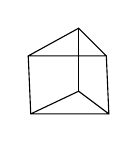
\begin{tikzpicture}[x=.032cm,y=-.032cm,line cap=round,line join=round]
\draw (0,11) -- (31,11) -- (20,0) -- cycle;
\draw (1,34) -- (32,34) -- (20,25) -- cycle;
\draw (0,11) -- (1,34);
\draw (31,11) -- (32,34);
\draw (20,0) -- (20,25);


\end{tikzpicture}}
prismes doubles \hspace{2em} $45.8$
\figure{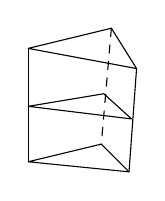
\begin{tikzpicture}[x=.032cm,y=-.032cm,line cap=round,line join=round]
\draw (0,8) -- (43,16) -- (33,0) -- cycle;
\draw (0,31) -- (41,36) -- (30,26) -- cycle;
\draw (0,53) -- (40,57) -- (29,46) -- cycle;
\draw (0,8) -- (0,53);
\draw (43,16) -- (40,57);
\draw[dashed] (33,0) -- (29,46);


\end{tikzpicture}}
antiprisme \unsure{torseur|torseur tordu|tordus} (\deleted{\unsure{appa|app|appelons}} \unsure{plan} projectif réel)
\margin{avec grain de sel pour le disque (faux) hexagonal qui \unsure{transforme|ferme} le \unsure{bandeau|ruban} de Möbius}
% slanted
\figure{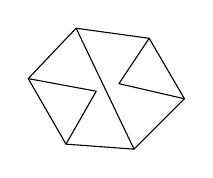
\begin{tikzpicture}[x=.032cm,y=-.032cm,line cap=round,line join=round]
\draw (0,20) -- (19,0) -- (48,4) -- (62,28) -- (42,48) -- (15,46) -- cycle;
\draw (19,0) -- (42,48);
\draw (0,20) -- (27,25) -- (15,46);
\draw (48,4) -- (36,22) -- (62,28);


\end{tikzpicture}}
pseudocube (cube avec $1$ arête contractée) \hspace{1em} $45.\deleted{\unsure{8|9}}.16.3=2^4 3^4 5$
\figure{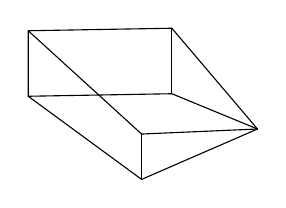
\begin{tikzpicture}[x=.032cm,y=-.032cm,line cap=round,line join=round]
\draw (0,1) -- (57,0) -- (91,40) -- (45,60) -- (0,27) -- cycle;
\draw (0,1) -- (45,42) -- (91,40);
\draw (45,42) -- (45,60);
\draw (0,27) -- (57,26) -- (91,40);
\draw (57,0) -- (57,26);


\end{tikzpicture}}
\uline{cubes} \hspace{1em} $27.10.\deleted{\unsure{4|1}}2=2^2.3^3.5$

dodécaèdre gauche \hspace{1em} $2^4.3^3=36.12=36.6.2$.

\diagram{\(\text{polygones}\quad\left\{\begin{array}{ll}
\text{carrés}&27.10.4=2^3 3^3 5\\
\text{pentagones}&36.6.12=2^5.3^4\\
\text{hexagones}&720=2^4.3^2.5
\end{array}\right.\)}

\figure{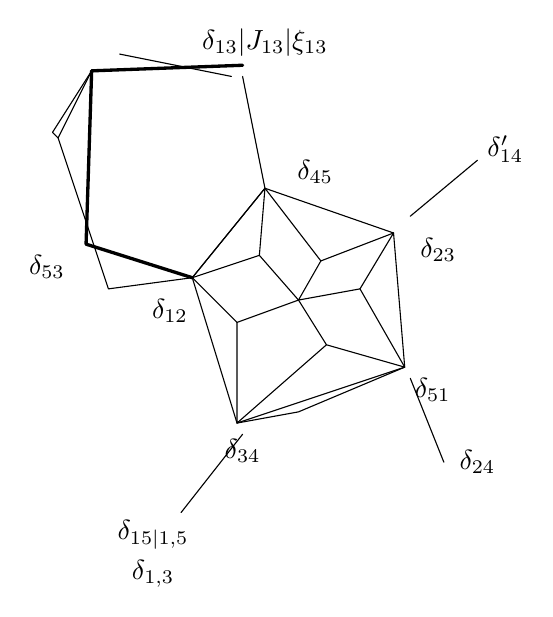
\begin{tikzpicture}[x=.071cm,y=-.071cm,line cap=round,line join=round]
\draw[very thick] (13,9) -- (40,8);
\draw[very thick] (13,9) -- (12,40) -- (31,46);
\draw (40,10) -- (44,30) -- (31,46) -- (16,48) -- (7,21) -- (13,9);
\draw (13,9) -- (6,20) -- (7,21);
\draw (18,6) -- (38,10);
\draw (44,30) -- (67,38) -- (69,62) -- (50,70) -- (39,72) -- (31,46) -- (44,30);
\draw (31,46) -- (43,42) -- (44,30);
\draw (43,42) -- (50,50) -- (39,54) -- (31,46);
\draw (39,54) -- (39,72) -- (55,58) -- (50,50);
\draw (44,30) -- (54,43) -- (67,38);
\draw (54,43) -- (50,50) -- (61,48) -- (67,38);
\draw (61,48) -- (69,62) -- (55,58);
\draw (69,62) -- (39,72);
\draw (70,35) -- (82,25);
\draw (40,74) -- (29,88);
\draw (70,64) -- (76,79);
\node[inner sep=.5pt] at (44,4) {$\unsure{\delta_{13}|J_{13}|\xi_{13}}$};
\node[inner sep=.5pt] at (53,27) {$\delta_{45}$};
\node[inner sep=.5pt] at (5,44) {$\delta_{53}$};
\node[inner sep=.5pt] at (27,52) {$\delta_{12}$};
\node[inner sep=.5pt] at (87,23) {$\delta'_{14}$};
\node[inner sep=.5pt] at (75,41) {$\delta_{23}$};
\node[inner sep=.5pt] at (74,66) {$\delta_{51}$};
\node[inner sep=.5pt] at (82,79) {$\delta_{24}$};
\node[inner sep=.5pt] at (40,77) {$\delta_{34}$};
\node[inner sep=.5pt] at (24,92) {$\delta_{\unsure{15|1,5}}$};
\node[inner sep=.5pt] at (24,99) {$\delta_{1,3}$};

\end{tikzpicture}}
$\underline{1\ 2\ 3\ 4\ \underline{5}}$
\figure{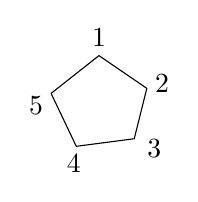
\begin{tikzpicture}[x=.032cm,y=-.032cm,line cap=round,line join=round]
\draw (4,16) -- (23,1) -- (42,14) -- (37,34) -- (14,37) -- cycle;
\node[inner sep=.5pt] at (23,-6) {$1$};
\node[inner sep=.5pt] at (48,12) {$2$};
\node[inner sep=.5pt] at (45,38) {$3$};
\node[inner sep=.5pt] at (13,44) {$4$};
\node[inner sep=.5pt] at (-2,21) {$5$};

\end{tikzpicture}}
\figure{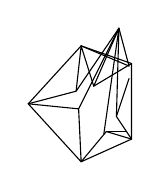
\begin{tikzpicture}[x=.032cm,y=-.032cm,line cap=round,line join=round]
\draw (0,30) -- (21,7) -- (41,14) -- (41,44) -- (21,53) -- cycle;
\draw (0,30) -- (19,25) -- (21,7) -- (26,23) -- (41,14);
\draw (0,30) -- (20,32) -- (21,53) -- (31,41) -- (41,44);
\draw (20,32) -- (36,0) -- (30,42);
\draw (19,25) -- (36,0) -- (35,35) -- (41,44);
\draw (26,23) -- (36,0) -- (40,15);
\draw (21,7) -- (40,15);
\draw (31,41) -- (39,41);
\draw (35,35) -- (40,20);


\end{tikzpicture}}
\figure{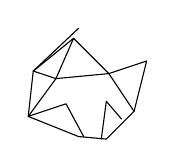
\begin{tikzpicture}[x=.032cm,y=-.032cm,line cap=round,line join=round]
\draw (2,17) -- (18,4) -- (32,18) -- (47,13) -- (42,33) -- (31,44) -- (20,43) -- (0,35) -- cycle;
\draw (2,17) -- (11,20) -- (18,4);
\draw (11,20) -- (0,35) -- (15,30) -- (22,43);
\draw (11,20) -- (32,18) -- (42,33);
\draw (29,44) -- (31,29) -- (37,36);
\draw (2,17) -- (20,0);


\end{tikzpicture}}
\figure{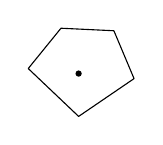
\begin{tikzpicture}[x=.032cm,y=-.032cm,line cap=round,line join=round]
\draw (0,16) -- (13,0) -- (34,1) -- (42,20) -- (20,35) -- cycle;

\fill (20,18) circle (.04cm);
\end{tikzpicture}}
$\delta_{56}\ \delta_{26}.\delta_{46}\ \delta_{16}\ \delta_{36}$
\[
\left|\begin{matrix}\delta_6\\\delta'_6\end{matrix}\right.\qquad
\deleted{\delta_{\unsure{123|23}}}\ 
\underbrace{\delta_{12}\ \delta_{34}\ \delta_{51}\ \delta_{23}}_{\text{pentagones}}\ \delta_{45}
\qquad 5.2\qquad 4!/2=
\]
\[
\begin{aligned}
2^5.3^4&=36.6.12\\
2^{8}\unsure{4|.}.5&\quad\text{\uline{aut.}}
\end{aligned}
\]

% The following block is upside down on the sheet and has long diagonal cancellation strokes.
\deleted{
\diagram{\(\begin{array}{rll}
 &C&I\amalg I\amalg\unsure{\mathfrak P_2|\mathscr P_2}(I)\\
 &&\delta_i\qquad\delta'_i\qquad\delta_{ij}\\
27\mid&\mathbb Z[C]&c.c'=\begin{cases}-1&\text{si }c=c'\\0&\text{si }c\ne c'\quad c,c'\text{ non liés}\\1&\text{si }c\ne c',\quad c',c''\text{ liés}\end{cases}\\
 &\downarrow&\\
7&\widehat E(C)&\underbrace{\delta_1,--\delta_6\quad\unsure{\eta|y}}_{\lambda.\deleted{\unsure{\delta|z|\sum}}\delta=1}=\delta_{ij}+\delta_i+\delta_j\qquad i\ne j\\
 &\rotatebox{90}{$\ni$}&\\
 &\lambda&\\
6&E(C)=\lambda^\perp&\\
 &\multicolumn{2}{l}{\{\delta'-\delta\mid\delta,\delta'\in C,\quad\delta,\delta'\text{ non liés}\}}\\
72&&\dfrac{\overset{\frown}{27.16}}6=72
\end{array}\)}
\figure{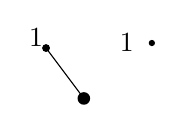
\begin{tikzpicture}[x=.032cm,y=-.032cm,line cap=round,line join=round]
\draw (4,5) -- (19,25);
\node[inner sep=.5pt] at (0,1) {$1$};
\node[inner sep=.5pt] at (36,3) {$1$};
\fill (4,5) circle (.05cm) (19,25) circle (.08cm) (46,3) circle (.04cm);
\end{tikzpicture}}
\[
\deleted{\begin{aligned}
&\sum_{b\in\unsure{\mathrm{Bas}|\mathrm{Bases}}(C)}\ \sum_{\beta\in\unsure{\mathcal P_{2,2,2}|\mathfrak P_{2,2,2}}(b)}\pi(\beta)\\
& b=\{\underbrace{b_1,\ },\underbrace{\ --\ },\underbrace{b_6}\}
\end{aligned}}
\]
\[
\begin{aligned}
b&=\{(b_i)_{1\leq i\unsure{\in|\leq}6}\} &\underbrace{b'_i-b_i}&=r_b\\
b'&=\{(b'_i)_{1\leq i\leq6}\}
\end{aligned}
\]
}
% archive sheet number: 77
\scanpage{79}
\figure{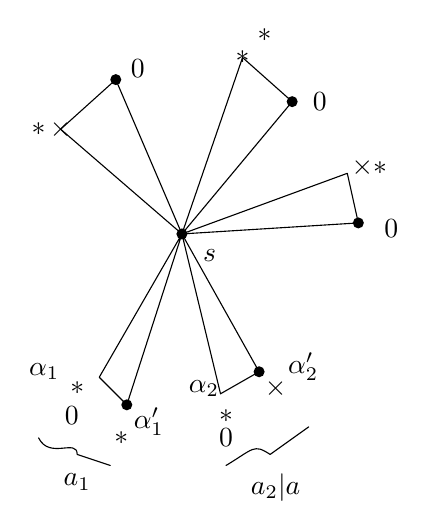
\begin{tikzpicture}[x=.07cm,y=-.07cm,line cap=round,line join=round]
\draw (36,36) -- (14,17) -- (24,8) -- cycle;
\draw (36,36) -- (47,4) -- (56,12) -- cycle;
\draw (36,36) -- (66,25) -- (68,34) -- cycle;
\draw (36,36) -- (50,61) -- (43,65) -- cycle;
\draw (36,36) -- (26,67) -- (21,62) -- cycle;
\node[inner sep=.5pt] at (10,17) {$*$};
\node[inner sep=.5pt] at (14,17) {$\times$};
\node[inner sep=.5pt] at (28,6) {$0$};
\node[inner sep=.5pt] at (47,4) {$*$};
\node[inner sep=.5pt] at (51,0) {$*$};
\node[inner sep=.5pt] at (61,12) {$0$};
\node[inner sep=.5pt] at (70,24) {$\times *$};
\node[inner sep=.5pt] at (74,35) {$0$};
\node[inner sep=.5pt] at (41,40) {$s$};
\node[inner sep=.5pt] at (11,61) {$\alpha_1$};
\node[inner sep=.5pt] at (17,64) {$*$};
\node[inner sep=.5pt] at (16,69) {$0$};
\node[inner sep=.5pt] at (30,70) {$\alpha'_1$};
\node[inner sep=.5pt] at (25,73) {$*$};
\node[inner sep=.5pt] at (53,64) {$\times$};
\node[inner sep=.5pt] at (58,60) {$\alpha'_2$};
\node[inner sep=.5pt] at (40,64) {$\alpha_2$};
\node[inner sep=.5pt] at (44,69) {$*$};
\node[inner sep=.5pt] at (44,73) {$0$};
\node[inner sep=.5pt] at (17,81) {$a_1$};
\node[inner sep=.5pt] at (53,82) {$\unsure{a_2|a}$};
\foreach \x/\y in {24/8,56/12,68/34,36/36,50/61,26/67}{\fill (\x,\y) circle (.07cm);}
\draw (10,73) .. controls (12,77) and (17,73) .. (17,76) -- (23,78);
\draw (44,78) .. controls (49,75) and (49,74) .. (52,76) -- (59,71);
\end{tikzpicture}}
\[
\begin{array}{l}M\subset\mathbb F_2^Q\\[-.3ex]\ \backslash\,P\end{array}
\]
\diagram{\begin{tikzcd}[ampersand replacement=\&,column sep=.5em,row sep=.5em]
\& {} \arrow[-]{r} \& {}\\
{} \arrow{ur} \arrow{r} \& {} \arrow{ur}\&
\end{tikzcd}}
$Q$ ens de card $5$

$I\unsure{\subset|\in} Q$ ens de cardinal $2$
\[
\begin{array}{l@{\qquad}l@{\qquad}l}
e_i\in M&e_1,e_2\quad e_1+e_2&\\
\unsure{P|R}&e'_1=e_2+e_3+e_4+e_5&e_i+\mathbb{1}\qquad e_j+\mathbb{1}\\
&e'_2=e_1+e_3+e_4+e_5&e_i-e_j+\unsure{\mathbb Z|2}\\
&e'_1+e'_2=e_1+e_2&
\end{array}
\]
\figure{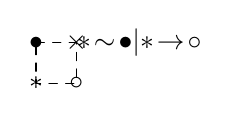
\begin{tikzpicture}[x=.032cm,y=-.032cm,line cap=round,line join=round]
\draw[dashed] (0,0) -- (16,0) -- (16,16) -- (0,16) -- cycle;
\node[inner sep=.5pt] at (0,0) {$\bullet$};
\node[inner sep=.5pt] at (16,0) {$\times$};
\node[inner sep=.5pt] at (0,16) {$*$};
\node[inner sep=.5pt] at (16,16) {$\circ$};
\node[inner sep=.5pt] at (41,0) {$\deleted{\unsure{*\!\sim\!\bullet|*\!\to\!\circ}}$};

\end{tikzpicture}}
\[
 e_i+\mathbb{1},\ e_j+\mathbb{1}\qquad e_i+e_j\qquad \mathbb F_2^I
\]
\diagram{\(\begin{array}{c|c|c|}&\alpha_1&\alpha'_1\\ \hline
\alpha_2&\circ&*\\ \hline
\alpha'_2&\times&\bullet\end{array}\)}
\diagram{\begin{tikzcd}[ampersand replacement=\&,row sep=.3em,column sep=1em]
\widetilde I^{\unsure{4|\ast}}\arrow{d}\&\\ I\&J\\ 2\&3
\end{tikzcd}}
\[
\begin{aligned}
&\deleted{\unsure{T|I}}\ \widetilde I\amalg(J\times\tau(\widetilde I/I))\\
&\underbrace{[0,1]}_{I_0}\amalg\underset{2}{I}_1\amalg(J\times I_1)
\end{aligned}
\]
\figure{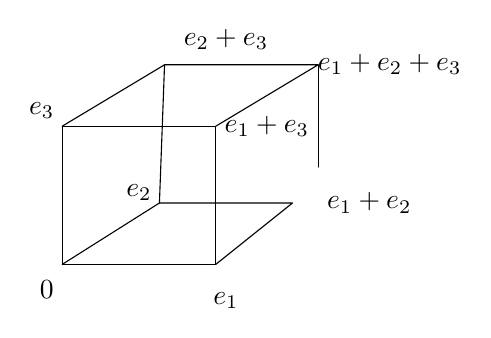
\begin{tikzpicture}[x=.065cm,y=-.065cm,line cap=round,line join=round]
\draw (0,21) -- (30,21) -- (30,48) -- (0,48) -- cycle;
\draw (0,21) -- (20,9) -- (50,9) -- (30,21);
\draw (0,48) -- (19,36) -- (45,36) -- (30,48);
\draw (19,36) -- (20,9);
\draw (50,9) -- (50,29);
\node[inner sep=.5pt] at (-3,53) {$0$};
\node[inner sep=.5pt] at (32,55) {$e_1$};
\node[inner sep=.5pt] at (15,34) {$e_2$};
\node[inner sep=.5pt] at (-4,18) {$e_3$};
\node[inner sep=.5pt] at (40,21) {$e_1+e_3$};
\node[inner sep=.5pt] at (60,36) {$e_1+e_2$};
\node[inner sep=.5pt] at (32,4) {$e_2+e_3$};
\node[inner sep=.5pt] at (64,9) {$e_1+e_2+e_3$};

\end{tikzpicture}}
\figure{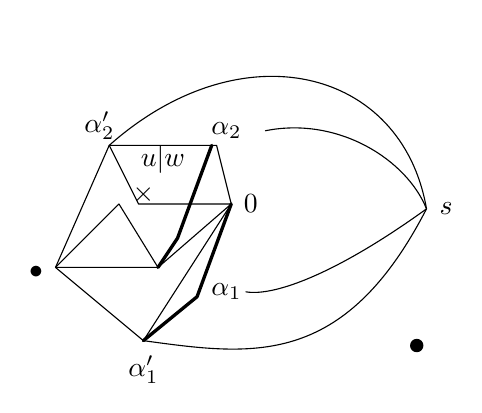
\begin{tikzpicture}[x=.062cm,y=-.062cm,line cap=round,line join=round]
\draw (4,37) -- (15,12) -- (37,12) -- (40,24) -- (22,52) -- cycle;
\draw (4,37) -- (25,37) -- (40,24);
\draw (15,12) -- (21,24) -- (40,24);
\draw (4,37) -- (17,24) -- (25,37);
\draw[very thick] (22,52) -- (33,43) -- (40,24);
\draw[very thick] (25,37) -- (29,31) -- (36,12);
\node[inner sep=.5pt] at (0,38) {$\bullet$};
\node[inner sep=.5pt] at (13,8) {$\alpha'_2$};
\node[inner sep=.5pt] at (39,9) {$\alpha_2$};
\node[inner sep=.5pt] at (44,24) {$0$};
\node[inner sep=.5pt] at (39,42) {$\alpha_1$};
\node[inner sep=.5pt] at (22,58) {$\alpha'_1$};
\node[inner sep=.5pt] at (84,25) {$s$};
\node[inner sep=.5pt] at (22,22) {$\times$};
\node[inner sep=.5pt] at (26,15) {$\unsure{u|w}$};
\draw (15,12) .. controls (42,-12) and (75,-4) .. (80,25) .. controls (63,58) and (44,55) .. (22,52);
\draw (47,9) .. controls (62,6) and (76,15) .. (80,25) .. controls (62,38) and (49,43) .. (43,42);
\fill (78,53) circle (.085cm);
\end{tikzpicture}}
\figure{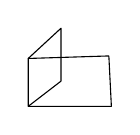
\begin{tikzpicture}[x=.032cm,y=-.032cm,line cap=round,line join=round]
\draw (0,12) -- (32,11) -- (33,31) -- (0,31) -- cycle;
\draw (0,12) -- (13,0) -- (13,21) -- (0,31);


\end{tikzpicture}}
\figure{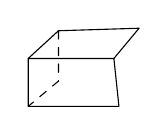
\begin{tikzpicture}[x=.032cm,y=-.032cm,line cap=round,line join=round]
\draw (0,12) -- (34,12) -- (36,31) -- (0,31) -- cycle;
\draw (0,12) -- (12,1) -- (44,0) -- (34,12);
\draw[dashed] (12,1) -- (12,21) -- (0,31);


\end{tikzpicture}}
\[
 e_1,\ e_2,\ e_3\qquad\deleted{\unsure{I\amalg I|2+2}}\ \mathbb F_2^J
\]
\figure{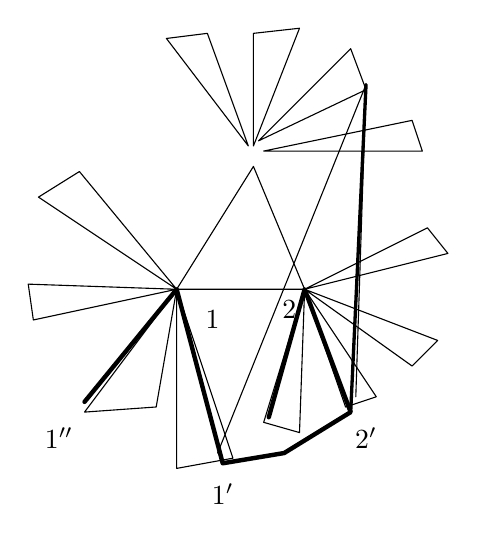
\begin{tikzpicture}[x=.065cm,y=-.065cm,line cap=round,line join=round]
\draw (30,56) -- (45,32) -- (55,56) -- cycle;
\draw (30,56) -- (3,38) -- (11,33) -- cycle;
\draw (30,56) -- (1,55) -- (2,62) -- cycle;
\draw (30,56) -- (12,80) -- (26,79) -- cycle;
\draw (30,56) -- (30,91) -- (41,89) -- cycle;
\draw (55,56) -- (79,44) -- (83,49) -- cycle;
\draw (55,56) -- (81,66) -- (76,71) -- cycle;
\draw (55,56) -- (69,77) -- (63,79) -- cycle;
\draw (55,56) -- (54,84) -- (47,82) -- cycle;
\draw (44,28) -- (28,7) -- (36,6) -- cycle;
\draw (45,28) -- (45,6) -- (54,5) -- cycle;
\draw (46,27) -- (64,9) -- (67,17) -- cycle;
\draw (47,29) -- (76,23) -- (78,29) -- cycle;
\draw (38,88) -- (67,16) -- (65,77);
\draw[ultra thick] (12,78) -- (30,56) -- (39,90) -- (51,88) -- (64,80) -- (55,56) -- (48,81);
\draw[very thick] (64,80) -- (67,16);
\node[inner sep=.5pt] at (37,62) {$1$};
\node[inner sep=.5pt] at (52,60) {$2$};
\node[inner sep=.5pt] at (7,85) {$1''$};
\node[inner sep=.5pt] at (39,96) {$1'$};
\node[inner sep=.5pt] at (67,85) {$2'$};

\end{tikzpicture}}
\[
\begin{aligned}
&3.2^6\qquad3.2^3\qquad3.2=6.\quad 2\\
&1''\quad\inserted{\text{lié : }1}\quad\text{non lié : }2'\ (\text{ou : }1')\\
&2''\ \deleted{\unsure{\sim|u}}\left\{\begin{array}{ll}\text{lié :}&2\\
\text{lié :}&1''.\\ \text{non lié :}&1',2'\end{array}\right.\\
&\left\{\begin{array}{l}\deleted{\text{lié}}\quad\deleted{\unsure{6|G|\in}}\unsure{\overline E(2)^*|E(2)^+|\widehat E(2)^*}\\
\text{lié : }1''\text{ et }\sigma1',\\
\ne\sigma2'\end{array}\right.
\end{aligned}
\]
\diagram{\begin{tikzcd}[ampersand replacement=\&,row sep=.6em,column sep=.9em]
\& w\&\sigma_4\&\\
\&u\arrow[-]{r}\arrow[-]{dl}\arrow[-]{d}\&v\arrow[-]{d}\arrow[-]{dr}\&\\
\alpha'_3\&\alpha_4\arrow[-]{r}\&\beta_4\&{}
\end{tikzcd}}
\diagram{\begin{tikzcd}[ampersand replacement=\&,row sep=.8em,column sep=.8em]
\&u\arrow[-]{r}\arrow[-]{dl}\arrow[-]{d}\&v\arrow[-]{dl}\arrow[-]{dr}\&\\
\alpha'_3\arrow[-]{r}\&\beta_3\arrow[-]{r}\&\alpha_4\arrow[-]{r}\&\beta_4
\end{tikzcd}}
\diagram{\begin{tikzcd}[ampersand replacement=\&,row sep=.6em,column sep=.5em]
\&\&\gamma_4\arrow[-]{d}\arrow[-]{dddll}\arrow[-,bend left=30]{ddd}\&\\
\&\&w\arrow[-]{dl}\arrow[-]{dr}\&\\
\&u\arrow[-]{rr}\arrow[-]{dl}\arrow[-]{d}\&\&v\arrow[-]{dl}\arrow[-]{d}\\
\alpha'_3\&\alpha_4\&\beta_3\&\beta_4
\end{tikzcd}}
\figure{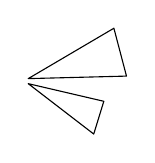
\begin{tikzpicture}[x=.032cm,y=-.032cm,line cap=round,line join=round]
\draw (0,20) -- (34,0) -- (39,19) -- cycle;
\draw (0,22) -- (30,29) -- (26,42) -- cycle;


\end{tikzpicture}}
\figure{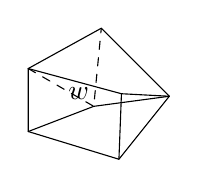
\begin{tikzpicture}[x=.032cm,y=-.032cm,line cap=round,line join=round]
\draw (0,16) -- (29,0) -- (56,27) -- (36,52) -- (0,41) -- cycle;
\draw (0,16) -- (37,26) -- (56,27);
\draw (37,26) -- (36,52);
\draw (0,41) -- (26,31) -- (56,27);
\draw[dashed] (0,16) -- (26,31) -- (29,0);
\node[inner sep=.5pt] at (20,26) {$w$};

\end{tikzpicture}}
\[
\begin{array}{c@{\qquad}cccc}
 \alpha'_3&\beta'_1&\beta'_2&\beta^{\unsure{\ast|1|\prime}}_3&\beta'_4\\
 \alpha'_4&\beta^{\unsure{\ast|1}}_1&\beta_2&\beta^1_3&\beta'_4
\end{array}\qquad 2.6.8
\]
% archive sheet number: 78
\scanpage{80}
\[
\underline{\underbrace{45.3}\,.\underbrace{32}\,.\underbrace{3}}:\unsure{\deleted{(3!3!)}|(3!3!)}=45.\deleted{\unsure{2|4}}.8\deleted{\unsure{2}}=2^3\,3^2\,5=360
\]
\[
\text{autom}\quad\underset{\substack{\Vert\\144}}{36.4}\ \big|\quad
(\unsure{\mathfrak S|\mathscr S}_3\times\mathfrak S_3).\mathfrak S_2\times\mathfrak S_2
\]
\figure{\begin{tikzpicture}[x=.032cm,y=-.032cm,line cap=round,line join=round]
\draw[gray!45] (1,37) -- (16,3) -- (46,39);


\end{tikzpicture}}
\figure{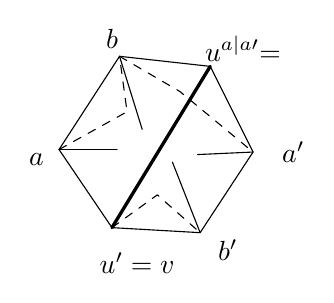
\begin{tikzpicture}[x=.032cm,y=-.032cm,line cap=round,line join=round]
\draw (7,40) -- (31,3) -- (67,7) -- (84,41) -- (63,73) -- (28,71) -- cycle;
\draw (7,40) -- (30,40);
\draw (62,42) -- (84,41);
\draw (31,3) -- (40,32);
\draw (52,45) -- (63,73);
\draw[very thick] (28,71) -- (67,7);
\draw[dashed] (7,40) -- (34,25) -- (31,3);
\draw[dashed] (28,71) -- (46,58) -- (63,73);
\draw[dashed] (31,3) -- (55,17) -- (84,41);
\node[inner sep=.5pt] at (-2,44) {$a$};
\node[inner sep=.5pt] at (28,-4) {$b$};
\node[inner sep=.5pt] at (80,0) {$u^{\unsure{a|a\prime}}{=}$};
\node[inner sep=.5pt] at (100,41) {$a'$};
\node[inner sep=.5pt] at (74,80) {$b'$};
\node[inner sep=.5pt] at (38,85) {$u'=v$};

\end{tikzpicture}}
\[
W_{\unsure{v|u}}(a).\quad w_u(b)\qquad
\underbrace{\unsure{\delta|J|\xi}_{12}\delta_{23}\delta_{34}}\ \underbrace{\delta_{45}\delta_{56}\delta_{64}}
\]
\[
w_v(a)-\{b\}\qquad\underline{\delta_i\delta'_{i'}}\quad 4\leq i\leq 6
\]
\figure{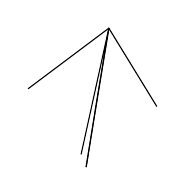
\begin{tikzpicture}[x=.032cm,y=-.032cm,line cap=round,line join=round]
\draw (0,24) -- (32,0) -- (51,31);
\draw (21,50) -- (32,0) -- (23,55);
\draw (23,55) -- (27,30) -- (32,0);


\end{tikzpicture}}
\figure{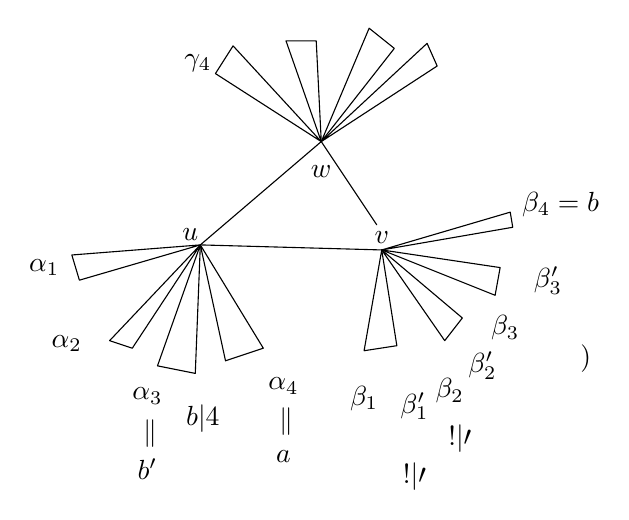
\begin{tikzpicture}[x=.032cm,y=-.032cm,line cap=round,line join=round]
\draw (45,81) -- (93,40) -- (115,73);
\draw (45,81) -- (117,83);
\draw (93,40) -- (51,13) -- (58,2) -- cycle;
\draw (93,40) -- (79,0) -- (91,0) -- cycle;
\draw (93,40) -- (112,-5) -- (122,3) -- cycle;
\draw (93,40) -- (135,1) -- (139,10) -- cycle;
\draw (45,81) -- (-3,95) -- (-6,85) -- cycle;
\draw (45,81) -- (9,119) -- (18,122) -- cycle;
\draw (45,81) -- (28,129) -- (43,132) -- cycle;
\draw (45,81) -- (55,127) -- (70,122) -- cycle;
\draw (117,83) -- (168,68) -- (169,74) -- cycle;
\draw (117,83) -- (164,90) -- (162,101) -- cycle;
\draw (117,83) -- (149,110) -- (142,119) -- cycle;
\draw (117,83) -- (123,121) -- (110,123) -- cycle;
\node[inner sep=.5pt] at (41,77) {$u$};
\node[inner sep=.5pt] at (117,78) {$v$};
\node[inner sep=.5pt] at (93,52) {$w$};
\node[inner sep=.5pt] at (44,9) {$\gamma_4$};
\node[inner sep=.5pt] at (-17,90) {$\alpha_1$};
\node[inner sep=.5pt] at (-8,120) {$\alpha_2$};
\node[inner sep=.5pt] at (24,141) {$\alpha_3$};
\node[inner sep=.5pt] at (25,156) {$\Vert$};
\node[inner sep=.5pt] at (24,170) {$b'$};
\node[inner sep=.5pt] at (46,150) {$\unsure{b|4}$};
\node[inner sep=.5pt] at (78,137) {$\alpha_4$};
\node[inner sep=.5pt] at (79,151) {$\Vert$};
\node[inner sep=.5pt] at (78,165) {$a$};
\node[inner sep=.5pt] at (188,65) {$\beta_4=b$};
\node[inner sep=.5pt] at (183,95) {$\beta'_3$};
\node[inner sep=.5pt] at (166,114) {$\beta_3$};
\node[inner sep=.5pt] at (157,129) {$\beta'_2$};
\node[inner sep=.5pt] at (144,139) {$\beta_2$};
\node[inner sep=.5pt] at (130,145) {$\beta'_1$};
\node[inner sep=.5pt] at (110,142) {$\beta_1$};
\node[inner sep=.5pt] at (148,158) {$\unsure{!|\prime}$};
\node[inner sep=.5pt] at (130,173) {$\unsure{!|\prime}$};
\node[inner sep=.5pt] at (198,126) {$)$};

\end{tikzpicture}}
\figure{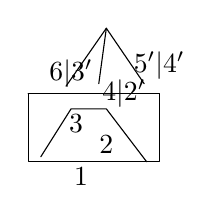
\begin{tikzpicture}[x=.032cm,y=-.032cm,line cap=round,line join=round]
\draw (2,27) -- (2,54) -- (54,54) -- (54,27);
\draw (2,27) -- (54,27);
\draw (7,52) -- (19,33) -- (33,33) -- (49,54);
\draw (17,24) -- (33,1) -- (48,23);
\draw (33,1) -- (30,23);
\node[inner sep=.5pt] at (23,60) {$1$};
\node[inner sep=.5pt] at (33,47) {$2$};
\node[inner sep=.5pt] at (21,39) {$3$};
\node[inner sep=.5pt] at (19,19) {$\unsure{6|3'}$};
\node[inner sep=.5pt] at (54,16) {$\unsure{5'|4'}$};
\node[inner sep=.5pt] at (40,27) {$\unsure{4|2'}$};

\end{tikzpicture}}
\unsure{Antiprisme|antiprisme|pentaprismes} $\sim$ couples de 3-bases voisines \deleted{et} bijection entre les deux --- couple d'une bibase et d'une partition de type $(3,3)$, avec iso. des deux morceaux i.e. isom. de $I$ (ens à 6 él) comme produit d'une de 3 par une de 2
\figure{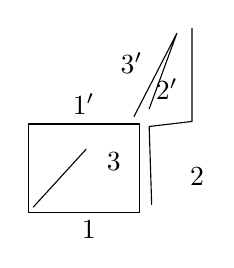
\begin{tikzpicture}[x=.032cm,y=-.032cm,line cap=round,line join=round]
\draw (0,38) -- (44,38) -- (44,73) -- (0,73) -- cycle;
\draw (2,71) -- (23,48);
\draw (49,70) -- (48,39) -- (65,37) -- (65,0);
\draw (42,35) -- (59,2) -- (48,32);
\node[inner sep=.5pt] at (24,80) {$1$};
\node[inner sep=.5pt] at (67,59) {$2$};
\node[inner sep=.5pt] at (34,53) {$3$};
\node[inner sep=.5pt] at (22,30) {$1'$};
\node[inner sep=.5pt] at (55,24) {$2'$};
\node[inner sep=.5pt] at (41,14) {$3'$};

\end{tikzpicture}}
\diagram{\begin{tikzcd}[ampersand replacement=\&,column sep=small,row sep=large]
a\arrow[r,dash]\arrow[d,dash] \& b\arrow[r,dash]\arrow[d,dash]\arrow[dl,dash] \& u\arrow[d,dash]\arrow[dl,dash]\\
a'\arrow[r,dash]\arrow[ur,dash,shift right] \& b'\arrow[r,dash] \& u'
\end{tikzcd}}
\par\noindent\rule{\linewidth}{.4pt}\par
\deleted{
\figure{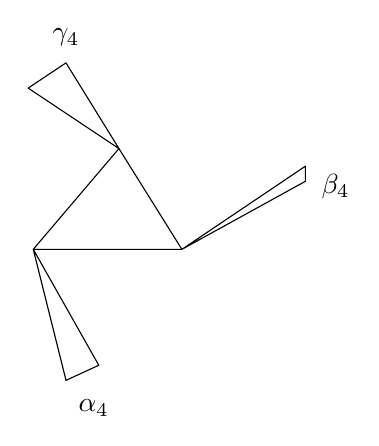
\begin{tikzpicture}[x=.032cm,y=-.032cm,line cap=round,line join=round]
\draw (7,74) -- (41,34) -- (66,74) -- cycle;
\draw (41,34) -- (5,10) -- (20,0) -- cycle;
\draw (66,74) -- (115,41) -- (115,47) -- cycle;
\draw (7,74) -- (20,126) -- (33,120) -- cycle;
\node[inner sep=.5pt] at (20,-10) {$\gamma_4$};
\node[inner sep=.5pt] at (127,49) {$\beta_4$};
\node[inner sep=.5pt] at (31,137) {$\alpha_4$};

\end{tikzpicture}}
\[
\begin{aligned}
U\mid P_u&=\mathrm{id} & V\unsure{\mid P_v)|(P_v)}&=\mathrm{id} & W(P_w)&=\mathrm{id}\\
U_{\deleted{\unsure{u|4}}}(\alpha_4)&=\alpha_4 & V\unsure{\mid(\beta_4)|(\beta_4)}&=\beta_4 & W(\gamma_4)&=\gamma_4
\end{aligned}
\]
\[
UVW\in\{1,\sigma\}\quad\overset{?}{\Longrightarrow}\quad U,V,W=1
\]
\diagram{\begin{tikzcd}[ampersand replacement=\&,row sep=small,column sep=small]
\&\unsure{K|\mathcal K|C}\arrow[r]\arrow[dl]\arrow[d]\arrow[dr]\& V\times V\times V\\
N_1\arrow[dr,equal] \& N_2\arrow[d,equal] \& N_3\arrow[dl,equal]\\
\&C\&
\end{tikzcd}}
\[
\begin{array}{cc}J&I\\\unsure{\wr\Vert|\Vert|\simeq}&\Vert\\V^*&\{u,v,w\}\end{array}
\]
\[
\underset{9}{I\times\{0,1,2\}}\ \amalg\
\underset{3}{I}\times\underset{3}{J}\times\underset{2}{\mathrm{Circ}(I)}
\]
}
% archive sheet number: 79
\scanpage{81}
\deleted{
\figure{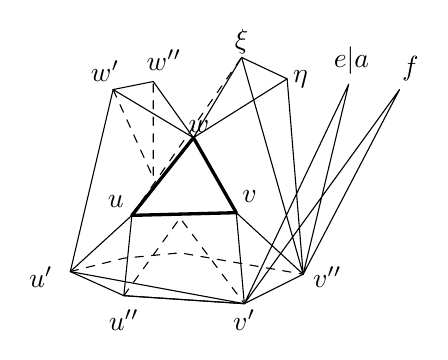
\begin{tikzpicture}[x=.034cm,y=-.034cm,line cap=round,line join=round]
\draw (35,62) -- (58,33) -- (74,61) -- cycle;
\draw[very thick] (35,62) -- (58,33) -- (74,61) -- (35,62);
\draw (58,33) -- (28,15) -- (43,12) -- (58,33) -- (76,3) -- (93,11) -- cycle;
\draw (28,15) -- (12,83) -- (35,62) -- (32,92) -- (77,95) -- (74,61) -- (99,84) -- (93,11);
\draw (12,83) -- (32,92) -- (77,95) -- (99,84);
\draw (12,83) -- (77,95);
\draw (76,3) -- (99,84) -- (116,13) -- (77,95) -- (135,15) -- (99,84);
\draw[dashed] (28,15) -- (43,48) -- (43,12);
\draw[dashed] (12,83) -- (32,78) -- (53,76) -- (99,84);
\draw[dashed] (32,92) -- (53,63) -- (77,95);
\draw[dashed] (35,62) -- (76,3);
\node[inner sep=.5pt] at (29,57) {$u$};
\node[inner sep=.5pt] at (79,55) {$v$};
\node[inner sep=.5pt] at (60,29) {$w$};
\node[inner sep=.5pt] at (1,85) {$u'$};
\node[inner sep=.5pt] at (32,101) {$u''$};
\node[inner sep=.5pt] at (77,101) {$v'$};
\node[inner sep=.5pt] at (108,85) {$v''$};
\node[inner sep=.5pt] at (25,8) {$w'$};
\node[inner sep=.5pt] at (47,4) {$w''$};
\node[inner sep=.5pt] at (76,-3) {$\xi$};
\node[inner sep=.5pt] at (98,11) {$\eta$};
\node[inner sep=.5pt] at (117,4) {$\unsure{e|a}$};
\node[inner sep=.5pt] at (139,7) {$f$};

\end{tikzpicture}}
\uline{Lemme}\quad $[u,v,w\ \text{triangle}]$ $u,v$ liés
\[
\begin{aligned}
u',u''&\ \text{liés à }u\quad(\text{et }\ne u,w,w\unsure{^*|\! \text{t}},\ \text{i.e. non liés à }v)\\
v',v''&\ \text{--- }v\quad(\text{---})\\
u',u''&\ \text{liés à chaque }v',v''\\[2pt]
\left\{\begin{array}{l}u',v',w'\ \text{triangle}\\u'',v'',w''\ \text{---}\end{array}\right. &\qquad \not\Rightarrow
\end{aligned}
\]
\figure{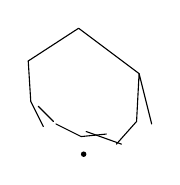
\begin{tikzpicture}[x=.032cm,y=-.032cm,line cap=round,line join=round]
\draw (2,21) -- (22,8) -- (46,26);
\draw (2,21) -- (3,37) -- (8,47);
\draw (6,39) -- (12,45);
\draw (13,46) -- (23,51) -- (33,50);
\draw (25,49) -- (39,54);
\draw (37,54) -- (45,45) -- (46,26) -- (51,46);

\fill (24,58) circle (1pt);
\end{tikzpicture}}
\figure{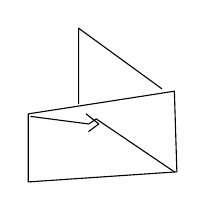
\begin{tikzpicture}[x=.032cm,y=-.032cm,line cap=round,line join=round]
\draw (3,34) -- (61,25) -- (62,57) -- (3,61) -- cycle;
\draw (23,30) -- (23,0) -- (56,24);
\draw (4,35) -- (27,38) -- (30,36) -- (61,57);
\draw (26,34) -- (31,38) -- (27,41);


\end{tikzpicture}}
\figure{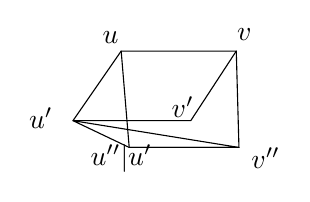
\begin{tikzpicture}[x=.034cm,y=-.034cm,line cap=round,line join=round]
\draw (5,29) -- (23,3) -- (66,3) -- (49,29) -- cycle;
\draw (23,3) -- (26,39) -- (67,39) -- (66,3);
\draw (5,29) -- (26,39) -- (67,39) -- cycle;
\node[inner sep=.5pt] at (19,-2) {$u$};
\node[inner sep=.5pt] at (69,-3) {$v$};
\node[inner sep=.5pt] at (-7,28) {$u'$};
\node[inner sep=.5pt] at (46,24) {$v'$};
\node[inner sep=.5pt] at (23,43) {$\deleted{\unsure{u''|u'}}$};
\node[inner sep=.5pt] at (77,43) {$v''$};

\end{tikzpicture}}
\figure{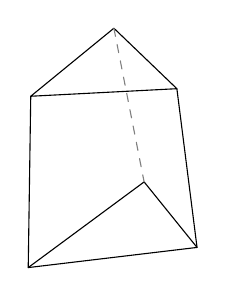
\begin{tikzpicture}[x=.032cm,y=-.032cm,line cap=round,line join=round]
\draw (1,27) -- (34,0) -- (59,24) -- cycle;
\draw (1,27) -- (0,95) -- (67,87) -- (59,24);
\draw (0,95) -- (46,61) -- (67,87);

\draw[gray,dashed] (34,0)--(46,61);
\end{tikzpicture}}
\figure{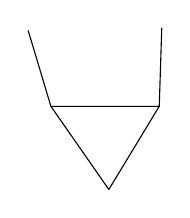
\begin{tikzpicture}[x=.032cm,y=-.032cm,line cap=round,line join=round]
\draw (0,1) -- (9,31) -- (52,31) -- (53,0);
\draw (9,31) -- (32,64) -- (52,31);


\end{tikzpicture}}
\figure{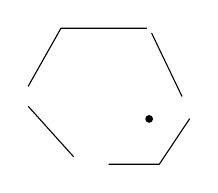
\begin{tikzpicture}[x=.032cm,y=-.032cm,line cap=round,line join=round]
\draw (1,26) -- (14,3) -- (48,3);
\draw (50,5) -- (62,30);
\draw (65,39) -- (53,57) -- (33,57);
\draw (19,54) -- (1,34);

\fill (49,39) circle (1.4pt);
\end{tikzpicture}}
\figure{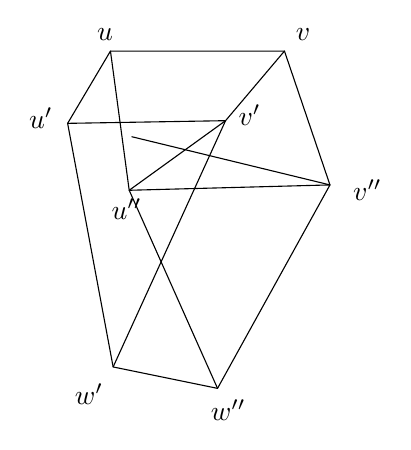
\begin{tikzpicture}[x=.034cm,y=-.034cm,line cap=round,line join=round]
\draw (1,29) -- (17,2) -- (82,2) -- (99,52) -- (57,128) -- (18,120) -- cycle;
\draw (17,2) -- (24,54) -- (99,52);
\draw (1,29) -- (60,28) -- (82,2);
\draw (24,54) -- (60,28);
\draw (25,34) -- (99,52);
\draw (24,54) -- (57,128);
\draw (18,120) -- (60,28);
\node[inner sep=.5pt] at (15,-4) {$u$};
\node[inner sep=.5pt] at (89,-4) {$v$};
\node[inner sep=.5pt] at (-9,27) {$u'$};
\node[inner sep=.5pt] at (23,61) {$u''$};
\node[inner sep=.5pt] at (69,26) {$v'$};
\node[inner sep=.5pt] at (113,54) {$v''$};
\node[inner sep=.5pt] at (9,130) {$w'$};
\node[inner sep=.5pt] at (61,136) {$w''$};

\end{tikzpicture}}
\figure{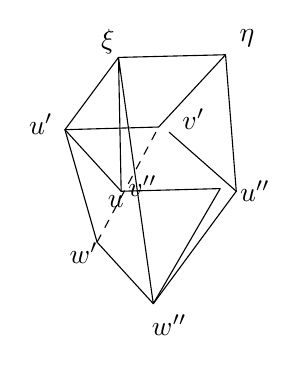
\begin{tikzpicture}[x=.034cm,y=-.034cm,line cap=round,line join=round]
\draw (1,30) -- (21,3) -- (61,2) -- (65,53) -- (34,95) -- (13,72) -- cycle;
\draw (1,30) -- (36,29) -- (61,2);
\draw (21,3) -- (22,53) -- (59,52) -- (34,95) -- cycle;
\draw (1,30) -- (22,53);
\draw (40,31) -- (65,53);
\draw[dashed] (13,72) -- (36,29);
\node[inner sep=.5pt] at (17,-3) {$\xi$};
\node[inner sep=.5pt] at (69,-4) {$\eta$};
\node[inner sep=.5pt] at (-8,28) {$u'$};
\node[inner sep=.5pt] at (49,26) {$v'$};
\node[inner sep=.5pt] at (20,57) {$u$};
\node[inner sep=.5pt] at (30,51) {$v''$};
\node[inner sep=.5pt] at (72,53) {$u''$};
\node[inner sep=.5pt] at (8,76) {$w'$};
\node[inner sep=.5pt] at (40,103) {$w''$};

\end{tikzpicture}}
\figure{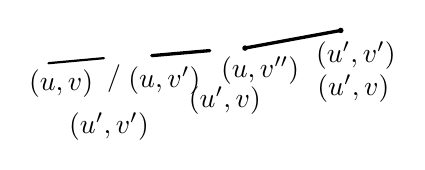
\begin{tikzpicture}[x=.032cm,y=-.032cm,line cap=round,line join=round]
\draw[thick] (3,14) -- (25,12);
\draw[very thick] (44,11) -- (67,9);
\draw[very thick] (81,8) -- (119,1);
\node[inner sep=.5pt] at (8,22) {$(u,v)$};
\node[inner sep=.5pt] at (29,20) {$/$};
\node[inner sep=.5pt] at (27,39) {$(u',v')$};
\node[inner sep=.5pt] at (49,21) {$(u,v')$};
\node[inner sep=.5pt] at (73,29) {$(u',v)$};
\node[inner sep=.5pt] at (87,17) {$(u,v'')$};
\node[inner sep=.5pt] at (125,11) {$(u',v')$};
\node[inner sep=.5pt] at (124,24) {$(u',v)$};
\fill (81,8) circle (1pt);\fill (119,1) circle (1pt);
\end{tikzpicture}}
\figure{\begin{tikzpicture}[x=.032cm,y=-.032cm,line cap=round,line join=round]

\node[inner sep=.5pt] at (0,8) {$u$};
\node[inner sep=.5pt] at (22,27) {$u'$};
\node[inner sep=.5pt] at (151,25) {$v$};
\node[inner sep=.5pt] at (186,15) {$v'$};
\node[inner sep=.5pt] at (222,4) {$v''$};
\foreach \x/\y in {8/1,28/19,154/15,188/3,211/-8} {\fill (\x,\y) circle (1.4pt);}
\end{tikzpicture}}
\figure{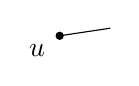
\begin{tikzpicture}[x=.032cm,y=-.032cm,line cap=round,line join=round]
\draw (5,3) -- (25,0);
\node[inner sep=.5pt] at (-4,9) {$u$};
\fill (5,3) circle (1.5pt);
\end{tikzpicture}}
\figure{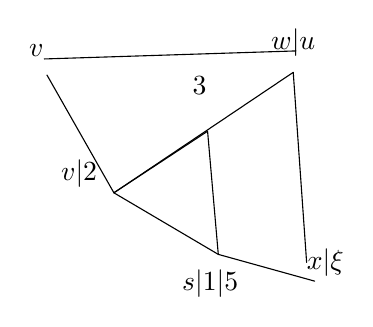
\begin{tikzpicture}[x=.034cm,y=-.034cm,line cap=round,line join=round]
\draw (0,3) -- (94,0);
\draw (1,9) -- (26,53) -- (93,8) -- (98,79);
\draw (26,53) -- (65,76) -- (101,86);
\draw (26,53) -- (61,30) -- (65,76);
\node[inner sep=.5pt] at (-3,0) {$v$};
\node[inner sep=.5pt] at (93,-3) {$\unsure{w|u}$};
\node[inner sep=.5pt] at (13,46) {$\unsure{v|2}$};
\node[inner sep=.5pt] at (58,13) {$3$};
\node[inner sep=.5pt] at (62,87) {$\unsure{s|1|5}$};
\node[inner sep=.5pt] at (105,79) {$\unsure{x|\xi}$};

\end{tikzpicture}}
\figure{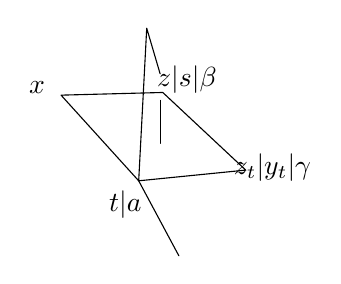
\begin{tikzpicture}[x=.034cm,y=-.034cm,line cap=round,line join=round]
\draw (0,25) -- (38,24) -- (69,53) -- (29,57) -- cycle;
\draw (29,57) -- (32,0) -- (37,17);
\draw (37,27) -- (37,43);
\draw (29,57) -- (44,85);
\node[inner sep=.5pt] at (-9,22) {$x$};
\node[inner sep=.5pt] at (47,19) {$\unsure{z|s|\beta}$};
\node[inner sep=.5pt] at (24,66) {$\deleted{\unsure{t|a}}$};
\node[inner sep=.5pt] at (79,52) {$\unsure{z_t|y_t|\gamma}$};

\end{tikzpicture}}
\figure{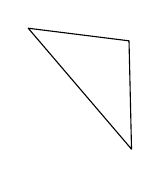
\begin{tikzpicture}[x=.032cm,y=-.032cm,line cap=round,line join=round]
\draw (0,0) -- (40,5) -- (41,48) -- cycle;


\end{tikzpicture}}
\figure{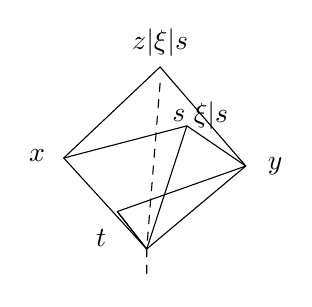
\begin{tikzpicture}[x=.034cm,y=-.034cm,line cap=round,line join=round]
\draw (1,40) -- (37,6) -- (69,43) -- (32,74) -- cycle;
\draw (1,40) -- (47,28) -- (69,43) -- (21,60) -- (32,74);
\draw (21,60) -- (32,74) -- (47,28);
\draw[dashed] (37,12) -- (32,74) -- (32,85);
\node[inner sep=.5pt] at (-9,39) {$x$};
\node[inner sep=.5pt] at (80,43) {$y$};
\node[inner sep=.5pt] at (15,70) {$t$};
\node[inner sep=.5pt] at (37,-3) {$\unsure{z|\xi|s}$};
\node[inner sep=.5pt] at (44,24) {$s$};
\node[inner sep=.5pt] at (56,24) {$\unsure{\xi|s}$};

\end{tikzpicture}}
\figure{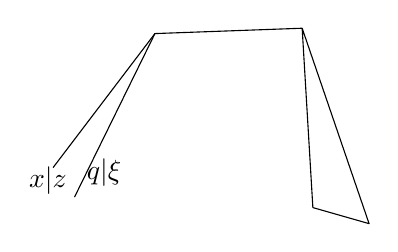
\begin{tikzpicture}[x=.034cm,y=-.034cm,line cap=round,line join=round]
\draw (1,55) -- (39,5) -- (94,3) -- (119,76) -- (98,70) -- (94,3);
\draw (9,66) -- (39,5);
\node[inner sep=.5pt] at (-1,60) {$\unsure{x|z}$};
\node[inner sep=.5pt] at (20,57) {$\unsure{q|\xi}$};

\end{tikzpicture}}
\figure{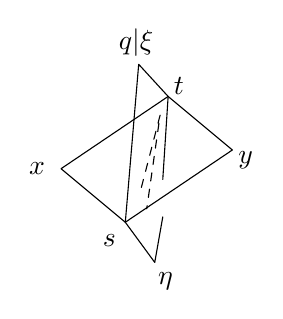
\begin{tikzpicture}[x=.034cm,y=-.034cm,line cap=round,line join=round]
\draw (3,42) -- (43,15) -- (67,35) -- (27,62) -- cycle;
\draw (27,62) -- (32,3) -- (43,15) -- (41,46);
\draw (27,62) -- (38,77) -- (41,60);
\draw[dashed] (33,49) -- (40,22) -- (35,57);
\node[inner sep=.5pt] at (-6,42) {$x$};
\node[inner sep=.5pt] at (72,39) {$y$};
\node[inner sep=.5pt] at (21,69) {$s$};
\node[inner sep=.5pt] at (47,11) {$t$};
\node[inner sep=.5pt] at (31,-5) {$\unsure{q|\xi}$};
\node[inner sep=.5pt] at (42,84) {$\eta$};

\end{tikzpicture}}
% margin note written sideways
\margin{$\gamma_1\quad\gamma'_2$}
% margin note written sideways
\margin{$\underbrace{\alpha_1\ \alpha'_2}\quad\underbrace{\beta'_1\ \beta_2}$}
% margin note written sideways
\margin{$\times\qquad\frown\ \frown\quad\underset{0}{V}\mathbin{\unsure{\alpha|\times}}V\times V$}
% margin note written sideways
\margin{$\begin{array}{ccccc}\alpha_1&\overset{?}{\beta'_1}&\beta_2&\beta_3&\beta_4\\ \unsure{\alpha_4|\alpha'_4}&\beta'_1&\beta'_2,&\beta'_3,&\beta_4\end{array}$}
% written sideways
\figure{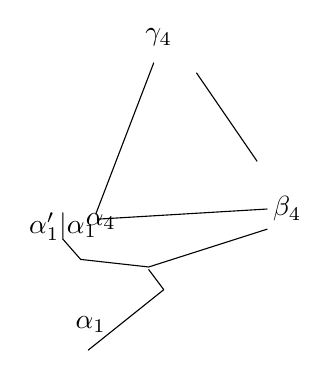
\begin{tikzpicture}[x=.032cm,y=-.032cm,line cap=round,line join=round]
\draw (0,73) -- (23,13);
\draw (40,17) -- (64,52);
\draw (1,75) -- (68,71);
\draw (-13,83) -- (-6,91) -- (21,94) -- (68,79);
\draw (21,95) -- (27,103) -- (-3,127);
\node[inner sep=.5pt] at (25,3) {$\gamma_4$};
\node[inner sep=.5pt] at (2,76) {$\alpha_4$};
\node[inner sep=.5pt] at (76,71) {$\beta_4$};
\node[inner sep=.5pt] at (-13,78) {$\deleted{\unsure{\alpha'_1|\alpha_1}}$};
\node[inner sep=.5pt] at (-2,117) {$\alpha_1$};

\end{tikzpicture}}
% margin note written sideways
\margin{$\begin{array}{cccc}\beta'_1&\beta_2&\beta_3&\underline{\beta_4}\\\beta_1&&&\end{array}$}
}
% archive sheet number: 80
\scanpage{82}
\figure{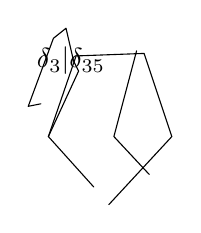
\begin{tikzpicture}[x=.032cm,y=-.032cm,line cap=round,line join=round]
\draw (9,43) -- (20,11) -- (47,10) -- (58,43) -- (33,70);
\draw (9,43) -- (27,63);
\draw (44,9) -- (35,43) -- (49,58);
\draw (6,30) -- (1,31) -- (11,4) -- (16,0) -- (19,13) -- (21,17) -- (9,43);
\node[inner sep=.5pt] at (18,13) {$\deleted{\unsure{\delta_3|\delta_{35}}}$};

\end{tikzpicture}}
\figure{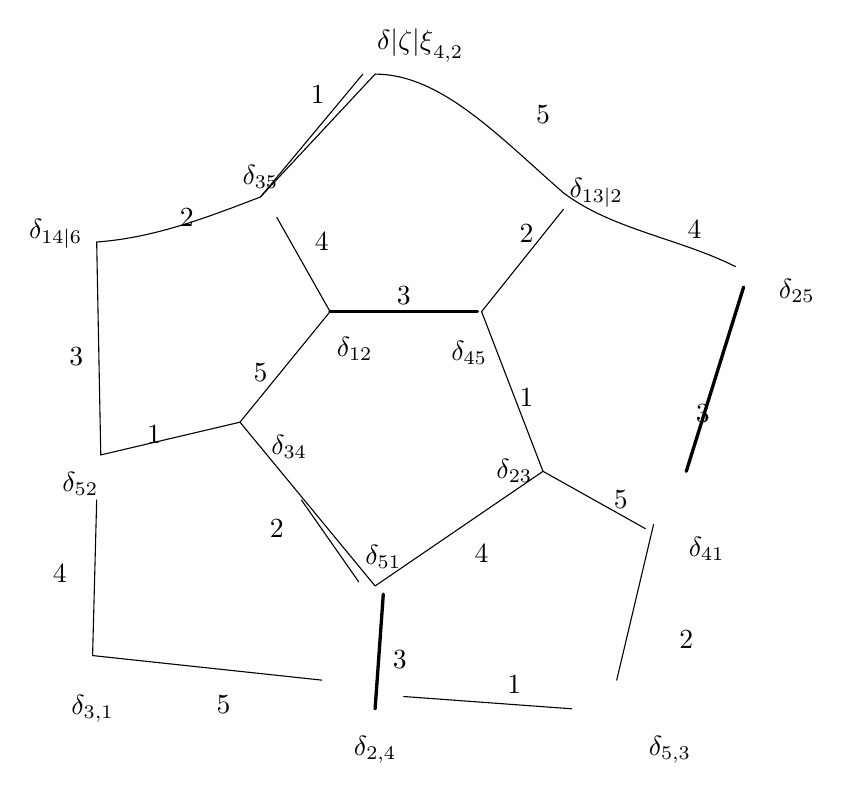
\begin{tikzpicture}[x=.052cm,y=-.052cm,line cap=round,line join=round]
\draw (12,46) .. controls (26,45) and (39,40) .. (52,35) -- (80,5);
\draw (80,5) .. controls (96,5) and (110,20) .. (126,34) .. controls (138,43) and (154,45) .. (168,52);
\draw (12,46) -- (13,98) -- (47,90);
\draw (12,109) -- (11,147) -- (67,153);
\draw (87,157) -- (128,160);
\draw (139,153) -- (148,115);
\draw[very thick] (156,102) -- (170,57);
\draw (126,38) -- (106,63);
\draw[very thick] (105,63) -- (69,63);
\draw (69,63) -- (56,40);
\draw (69,63) -- (47,90) -- (80,130) -- (121,102) -- (106,63);
\draw (121,102) -- (146,116);
\draw[very thick] (82,132) -- (80,160);
\draw[thin] (52,35) -- (77,5);
\draw[thin] (62,109) -- (76,129);
\node[inner sep=.5pt] at (91,-2) {$\unsure{\delta|\zeta|\xi}_{4,2}$};
\node[inner sep=.5pt] at (52,30) {$\delta_{35}$};
\node[inner sep=.5pt] at (134,34) {$\delta_{1\unsure{3|2}}$};
\node[inner sep=.5pt] at (183,58) {$\delta_{25}$};
\node[inner sep=.5pt] at (2,44) {$\delta_{1\unsure{4|6}}$};
\node[inner sep=.5pt] at (8,105) {$\delta_{52}$};
\node[inner sep=.5pt] at (75,72) {$\delta_{12}$};
\node[inner sep=.5pt] at (103,73) {$\delta_{45}$};
\node[inner sep=.5pt] at (59,96) {$\delta_{34}$};
\node[inner sep=.5pt] at (114,102) {$\delta_{23}$};
\node[inner sep=.5pt] at (82,123) {$\delta_{51}$};
\node[inner sep=.5pt] at (161,121) {$\delta_{41}$};
\node[inner sep=.5pt] at (11,160) {$\delta_{3,1}$};
\node[inner sep=.5pt] at (80,170) {$\delta_{2,4}$};
\node[inner sep=.5pt] at (152,170) {$\delta_{5,3}$};
\node[inner sep=.5pt] at (66,10) {$1$};
\node[inner sep=.5pt] at (121,15) {$5$};
\node[inner sep=.5pt] at (34,40) {$2$};
\node[inner sep=.5pt] at (67,46) {$4$};
\node[inner sep=.5pt] at (117,44) {$2$};
\node[inner sep=.5pt] at (158,43) {$4$};
\node[inner sep=.5pt] at (87,59) {$3$};
\node[inner sep=.5pt] at (7,74) {$3$};
\node[inner sep=.5pt] at (26,93) {$1$};
\node[inner sep=.5pt] at (52,78) {$5$};
\node[inner sep=.5pt] at (117,84) {$1$};
\node[inner sep=.5pt] at (160,88) {$3$};
\node[inner sep=.5pt] at (56,116) {$2$};
\node[inner sep=.5pt] at (106,122) {$4$};
\node[inner sep=.5pt] at (140,109) {$5$};
\node[inner sep=.5pt] at (3,127) {$4$};
\node[inner sep=.5pt] at (43,159) {$5$};
\node[inner sep=.5pt] at (86,148) {$3$};
\node[inner sep=.5pt] at (114,154) {$1$};
\node[inner sep=.5pt] at (156,143) {$2$};

\end{tikzpicture}}
$1\ 4\ 6$
% archive sheet number: 81
\scanpage{83}
% Mirrored type shows through from the other face.
\[
\delta'_1-\delta_1=\delta'_2-\delta_2\qquad
\delta'_1\ne\delta'_2,\quad\delta'_1\ne\delta_1
\]
\[
\begin{aligned}
\underbrace{\delta'_1+\delta_2}&=\underbrace{\delta'_2\unsure{\cdot|+}\delta_1}\\
\delta'_1\ \text{lié à }\delta_2 &\qquad \delta'_2\ \text{lié à }\delta_1\\
\delta'_1&\ \text{lié ni à }\delta'_2\ \text{ni à }\delta_1
\end{aligned}
\]
\[
\begin{aligned}
\unsure{\delta|\zeta|\xi}_{ij}&=\unsure{\eta|y}-\delta_i-\delta_j\\
\sum\delta_{ij}&=15\eta-5\unsure{\zeta|\delta|\xi}=5\lambda
\end{aligned}
\]

différences de sommets

\textcircled{a} sommets non liés se groupent par paquets de 6 parmi les $27.16$ possibilités virtuelles, d'où 72 ``\unsure{racines|voisines}'' (de carré $-2$)

\textcircled{b} sommets liés donnent $27.10=270$ autres éléments \unsure{remarquables}, \inserted{distincts \unsure{correspondt|correspondent|correspondant} aux arcs} \deleted{\unsure{soit en}} (de carré $-4$), soit en tout 342 éléments \deleted{(de carré $-4$)}.

sommes de 2 sommets

\textcircled{a} sommets \deleted{non} liés ($\unsure{\Leftrightarrow|\equiv}$ arêtes) se groupent par paquets de 5 parmi les \deleted{\unsure{les}} $27.10/2=135$ possib. virtuelles, pour donner 27 sommes (d'augment 2) correspondent aux 27 ``\deleted{triangles}'' sommets car \unsure{formés|formées} par le sommet $\delta$ les 5 \deleted{\unsure{demi|som}} triangles adjoints, et les arêtes opposées
\[
\delta\longmapsto\lambda-\delta.
\]
\[
\begin{aligned}
\delta_i&\longrightarrow\underbrace{\delta'_j,\delta_{ij}}&
\delta'_j+\delta_{ij}&=2\eta-\unsure{\zeta|\delta|\xi}+\delta_j\\
&&&\quad{}+\eta-\delta_i-\delta_j\\
&&&=\deleted{\unsure{2\eta|3\eta}}\lambda-\delta_i
\end{aligned}
\]
\[
\begin{aligned}
\delta'_i &\longmapsto\underbrace{\delta_j,\delta_{ij}}&
\delta_j+\delta_{ij}&=\unsure{\eta|p}-\delta_j\\
&&&=\unsure{\ldotp\ \ldotp|\, ,\, -}
\end{aligned}
\]

\textcircled{b} \inserted{\unsure{paires de|couples de}} sommets non liés \inserted{(correspondent aux \unsure{bigons|bigones|bicycles} ponctués)} donnent $27.16/2=216$ autres sommes distinctes, faisant avec les précédentes
\[
27+216=243\ \text{éléments.}
\]

sommes de 3 sommets
% archive sheet number: 82
\scanpage{84}
{\itshape
% letterhead
UNIVERSITE DES SCIENCES\\
ET TECHNIQUES DU LANGUEDOC

M A T H E M A T I Q U E S

D.E.U.G. A Première Année

Option Mathématique

1976

\uline{Titre}\qquad Polyèdres réguliers

Ce ``cours'' est destiné aux étudiants disposés à trouver de l'amusement en faisant des choses mathématiques très élémentaires et ``visuelles'', pouvant servir d'introduction à plusieurs courants d'idées et types d'intuition importants de géométrie et de topologie $n$-dimensionnelle. Il ne sera d'aucune utilité pour la préparation d'autres certificats de mathématiques. Il n'y aura pas de travaux dirigés proprement dits, et les séances seront en partie consacrées à la réflexion collective sur des questions se présentant dans l'exposé, avec des volontaires venant éventuellement expliquer une démonstration au tableau. Pas d'exercices notés. Le cours est divisé en deux parties, qui seront développées simultanément, l'une par A. GROTHENDIECK, l'autre par C. CONTOU CARRERE. Ces parties sont dans une large mesure indépendantes l'une de l'autre. Il y sera question des choses suivantes :

I) \uline{Polyèdres} : Polygones plans, division des plans en deux parties (``th. de Jordan''), cas convexe. Polyèdres convexes, facettes du polyèdre convexe, combinatoire d'un polyèdre convexe. Dualité des polyèdres convexes ayant un point intérieur donné. Peut-être des notions sur les polyèdres pas nécessairement convexes.

II) \uline{Les cinq polyèdres réguliers} (``solides platoniciens''). Description métrique, description combinatoire, éventuellement description ``projective'' en termes de ``configurations'' de points, droites et plans. Etude de leurs groupes de symétrie, liens avec les ``groupes symétriques'' $\handwritten{\unsure{\mathfrak S|\mathscr S}}_3$, $\handwritten{\mathfrak S}_4$, $\handwritten{\mathfrak S}_5$ des permutations d'ensembles finis : 3,4,5 objets, et leurs sous-groupes.

On présuppose une familiarité raisonnable de l'étudiant avec la géométrie du plan et de l'espace, qu'on abordera dans des points de vue nouveaux pour lui, et avec la notion de groupe, dont le ``cours'' permettra une compréhension plus approfondie par l'examen détaillé d'exemples concrets.
}
% archive sheet number: 83
